\documentclass[12pt, letterpaper]{article}

\title{AA279c Project Report: Modeling the ISS}
\author{Toby J. Buckley}
\date{\today}




\usepackage{graphicx}
\usepackage{subcaption}
\usepackage{float}
\usepackage{amsmath}
\usepackage{pdfpages}
\usepackage{hyperref}
\usepackage{url}

\usepackage[margin=1in]{geometry}

\graphicspath{{./src/html/}}
\DeclareGraphicsExtensions{.pdf,.png,.jpg}



\makeatletter
\newcommand\urlfootnote@[1]{\footnote{\url@{#1}}}
\DeclareRobustCommand{\urlfootnote}{\hyper@normalise\urlfootnote@}
\makeatother

\linespread{1.25}





\begin{document}

\begin{titlepage}
	\maketitle
	\centering
	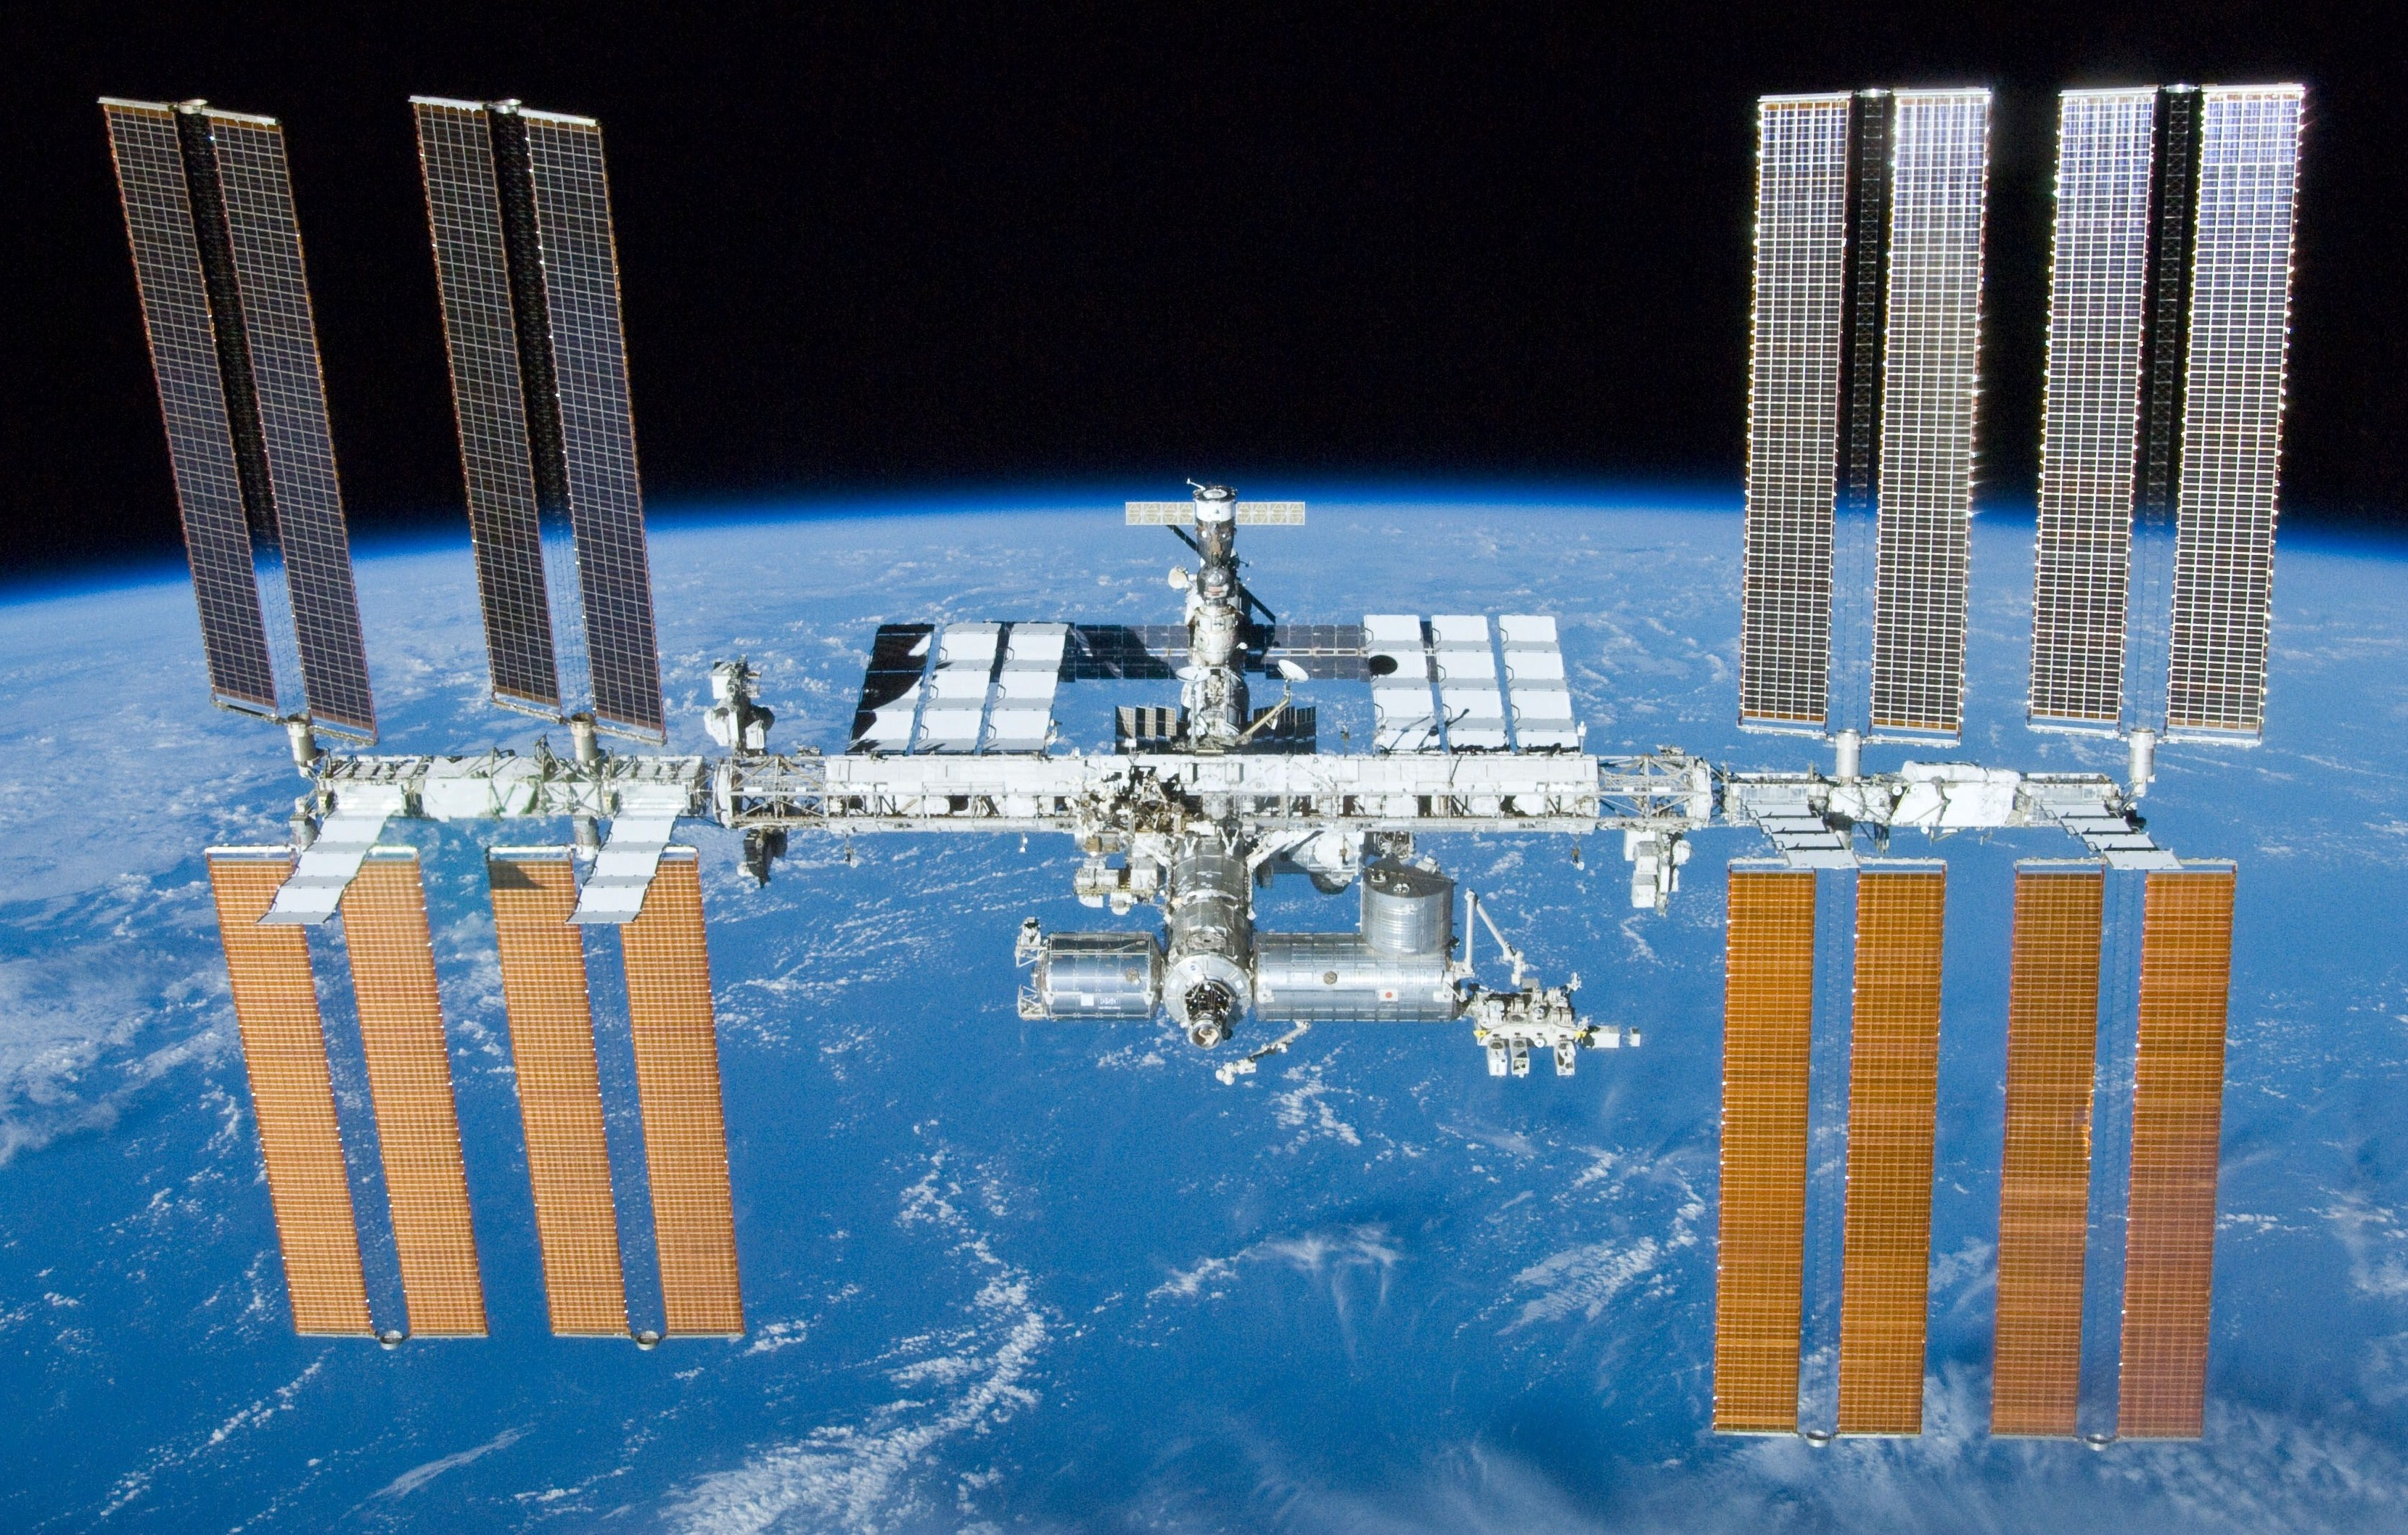
\includegraphics[width=\textwidth]{ISS}
\end{titlepage}






% 4 thrusters - 13.3 kg-f (29.3 lbf) https://www.quora.com/How-does-the-International-Space-Station-maintain-its-orbit-and-what-propellant-does-it-use


\section{Problem Set 1 - Mission Setup and Details.}
\subsection{Project Overview}
For this project the International Space Station (ISS) is modeled and explored, which orbits around the earth in low-earth-orbit (LEO). The ISS was first launched in 1998 and only fully completed in 2009. The full cost is estimated around 150 billion USD, making it the single-most expensive structure every created by man. In the nearly 20 years of operation, countless experiments have taken place onboard, dozens of astronauts have visited, and the total scientific value is immeasurable. The ISS is a tribute to humanity's ability to work together and has solidified its place in human history.



\begin{figure}[H]
	\centering
	\includegraphics[scale=0.8,width=\textwidth]{iss_config}
	\caption{ISS component breakdown.}
	\label{1:config}
\end{figure}

Fig. \ref{1:config} shows the exploded component view of the ISS. Over the course of its assembly parts were brought up by different rockets, the two most well known being the US Space Shuttle, and the Russian Soyuz. Sizing was done by referencing the ISS's wikipedia page\footnote{\url{https://en.wikipedia.org/wiki/Assembly_of_the_International_Space_Station}} as well as documents released by NASA\footnote{\url{https://www.nasa.gov/pdf/508318main_ISS_ref_guide_nov2010.pdf}}.


\begin{figure}[H]
	\centering
	\includegraphics[scale=0.8]{ps1_childs}
	\caption{Child creation code.}
	\label{1:code1}
\end{figure}

When putting together the data structure for the vehicle, I implemented a nested parent-child system, where each component of the ISS could be defined and attached with respect to the parent center. Fig. \ref{1:code1} shows how the different main components are defined. When information was missing, educated guesses on size were used.

In order to reduce complexity, only the largest components of the ISS were modeled. Structural elements such as the main truss, the pressurized cabin area, and solar panels were kept. Additionally, all body components are axis-aligned for ease of transformations and plotting.

Orbit propagation is performed using the two-body problem differential equation (below). This is derived using the standard Newton's second law approach assuming that the only bodies affecting each-other are the satellite and the orbiting body (Earth).

\begin{center}\includegraphics{ps1_2body}\end{center}


The two-body problem is modeled in Matlab Simulink which serves as the core of the environment simulator. The state is output in the earth-centered-inertial (ECI) frame and fed into the rest of the model. Fig. \ref{1:orbit} shows the model, which includes J2 effects and atmospheric drag. Due to the ISS's proximity to Earth, both of these greatly affect the orbit, and within only a couple orbits its clear that the satellite begins falling to earth.


\begin{figure}[H]
	\centering
	\includegraphics[scale=0.8,width=\textwidth]{ps1_orbitSim}
	\caption{Simulink model of the orbit propagator. Drag and J2 perturbation are included.}
	\label{1:orbit}
\end{figure}

When setting up the vehicle, the moment of inertia must be calculated for each component about a fixed point. In my code, each child automatically reports its inertia relative to the parent center, which is not necessarily the center of mass. Two transformations then take place; the first transforms the inertia relative to the true center of mass, and the second solves the principle axis eigenvalue problem. Eq. \ref{1:inertia1} \& \ref{1:eig1} show how these transformations are accomplished. For the eigenvalue problem, the eigenvalues are the principle axis inertia values, while the eigenvectors make up the unit triad which defines the rotation between the body and principle axes.

\begin{gather}
J_{ij} = I_{ij} + m(|R|^2\delta_{ij}-R_iR_j)
\label{1:inertia1} \\ 
(J-I*\lambda)A=0
\label{1:eig1}
\end{gather}

Below the moment of inertia tensor for the simplified ISS is shown, in both body and principle axes with respect to the center of mass. All computations are done using km, so these values are in $kg*km^2$.


\begin{equation}
J_b =\left(\begin{array}{ccc} 15.63 & 0 & -0.36\\ 0 & 6.43 & 0\\ -0.36 & 0 & 16.40 \end{array}\right), J_p =
\left(\begin{array}{ccc} 6.43 & 0 & 0\\ 0 & 15.49 & 0\\ 0 & 0 & 16.54 \end{array}\right)
\label{1:eqJ}
\end{equation}


Fig. \ref{1:iss} shows the full simplified vehicle. In the middle, at the center of mass there is the unit triad which rotates any vector from body to principle axis. Because the ISS is symmetric about the XZ plane, the y-component is hidden along the main truss. 

\begin{figure}[H]
	\centering
	\includegraphics[scale=0.8,trim={10mm, 5mm, 13mm, 3mm},clip]{ps1_01}
	\caption{Model of the ISS. Shown in blue, green, and red is the unit triad from body to principle.}
	\label{1:iss}
\end{figure}


In order to properly model atmospheric drag and gravity gradient, it's necessary to know the location of each children surface's barycenter and normal direction. Fig. \ref{1:iss_normal} shows the full vehicle with normal directions plotted at each surface' barycenter.

\begin{figure}[H]
	\centering
	\includegraphics[width=1.4\textwidth,trim={120mm, 20mm, 20mm, 10mm},clip]{iss_normals}
	\caption{The surface normals for each child are shown.}
	\label{1:iss_normal}
\end{figure}



The orbit propagation is demonstrated in Fig. \ref{1:orbit2}. Due to the proximity to Earth, the ISS travels at 4.76 miles/s and completes a single orbit in just around 90 minutes.


\begin{figure}[H]
	\centering
	\includegraphics[scale=0.8,trim={10mm, 0mm, 1mm, 0mm},clip]{ps1_02}
	\caption{Orbit propagation of ISS in LEO.}
	\label{1:orbit2}
\end{figure}





\section{Problem Set 2 - Conservation Laws, Ellipsoids of Rotational Motion, Euler equations}

The governing equation for the angular rates of a spacecraft is derived using the angular momentum version of Newton's second law, $M = \dot{H}$, where $H$ is the angular momentum. Below is the expanded version, as a function of the moment of inertia, $I$, and the angular velocity, $\omega$. It is assumed that the moment of inertia does not vary through the flight.

\begin{figure}[H]
	\centering
	\includegraphics[scale=0.6]{ps2_euler1}
\end{figure}

The explicit relation between $\dot{\omega}$ and $\omega$ is shown below. The moments, $M_i$ are modeled as perturbations. Notice that only the diagonal elements of moment of inertia are present. That's because we perform our analysis in the principle frame, in which all off-diagonal elements of the $I$ matrix are zero. This is the power of maintaining a transformation to the principle axis.

\begin{figure}[H]
	\centering
	\includegraphics[scale=0.6]{ps2_euler2}
\end{figure}

\begin{figure}[H]
	\centering
	\includegraphics[scale=0.6,width=0.6\textwidth]{ps2_eulerSim}
	\caption{Simulink model for the Euler equations.}
	\label{2:eulerSim}
\end{figure}

Fig. \ref{2:eulerSim} shows how the Euler equations are implemented in the simulink model. All calculations are done in the principle frame, so post-processing requires transformation to inertial frame. 

When validating the Euler equations, one can utilize the conservation of energy and angular momentum to ensure the integration is performed correctly. Below shows the energy and momentum ellipsoid equations. Motion is only physically possible when two closed lines form at the intersection of the two ellipsoids.

\begin{figure}[H]
	\centering
	\includegraphics[scale=0.6]{ps2_energyEll}
\end{figure}


\begin{figure}[H]
	\centering
	\includegraphics[scale=0.6]{ps2_momEll}
\end{figure}


\subsection{Rotation about arbitary direction}

For validation, the satellite is initiated with a random ang. vel. and allowed to propagate. After running the simulation, the output is post-processed to validate the results. A random starting velocity is generated and the euler equations propagate naturally. With no external torques, energy is conserved as shown in Fig. \ref{(2:angVelEnergy)}. The noise is due to numerical error from the simulation.

\begin{figure}[H]
	\centering
	\begin{subfigure}[b]{0.49\textwidth}
		\includegraphics[width=\textwidth,trim={10mm, 5mm, 13mm, 3mm},clip]{ps2_01}
	\end{subfigure}
	\begin{subfigure}[b]{0.49\textwidth}
		\includegraphics[width=\textwidth,trim={10mm, 5mm, 13mm, 3mm},clip]{ps2_02}
	\end{subfigure}
	\caption{Ang vel. and rotational energy.}
	\label{(2:angVelEnergy)}
\end{figure}

In Fig. \ref{2:ellipsoids} the momentum and energy ellipsoids are plotted for this simulation. Highlighted in orange and blue is the intersection. 

\begin{figure}[H]
	\centering
	\includegraphics[scale=0.9,trim={10mm, 5mm, 13mm, 3mm},clip]{ps2_03}
	\caption{Momentum and energy ellipsoids. The intersection is physically realizable.}
	\label{2:ellipsoids}
\end{figure}


\begin{figure}[H]
	\centering
	\begin{subfigure}[b]{0.32\textwidth}
		\includegraphics[width=\textwidth,trim={10mm, 5mm, 13mm, 3mm},clip]{ps2_04}
	\end{subfigure}
	\begin{subfigure}[b]{0.32\textwidth}
		\includegraphics[width=\textwidth,trim={10mm, 5mm, 13mm, 3mm},clip]{ps2_05}
	\end{subfigure}
	\begin{subfigure}[b]{0.32\textwidth}
		\includegraphics[width=\textwidth,trim={10mm, 5mm, 13mm, 3mm},clip]{ps2_06}
	\end{subfigure}
	\caption{Polhode in each plane.}
	\label{2:polhodePlanes}
\end{figure}

When the two ellipsoids are set equal to each-other, the resulting shape is described by eq. \ref{2:p1}-\ref{2:p3}. This produces an ellipse in the XY \& YZ planes, and a hyperbola in the XZ plane, as confirmed in Fig. \ref{2:polhodePlanes}.

\begin{gather}
\label{2:p1}
(I_y-I_x)I_yw_y^2+(I_z-I_x)I_zw_z^2=L^2-2TI_x \\
\label{2:p2}
(I_z-I_y)I_xw_x^2+(I_z-I_y)I_zw_z^2=L^2-2TI_y \\
\label{2:p3}
(I_x-I_z)I_xw_x^2+(I_y-I_z)I_yw_y^2=L^2-2TI_z
\end{gather}


\begin{figure}[H]
	\centering
	\begin{subfigure}[b]{0.32\textwidth}
		\includegraphics[width=\textwidth,trim={10mm, 5mm, 13mm, 3mm},clip]{ps2_07}
	\end{subfigure}
	\begin{subfigure}[b]{0.32\textwidth}
		\includegraphics[width=\textwidth,trim={10mm, 5mm, 13mm, 3mm},clip]{ps2_08}
	\end{subfigure}
	\begin{subfigure}[b]{0.32\textwidth}
		\includegraphics[width=\textwidth,trim={10mm, 5mm, 13mm, 3mm},clip]{ps2_09}
	\end{subfigure}
	\caption{Phase plane in each direction.}
	\label{2:phaseplane}
\end{figure}

Along with analyzing the energy and momentum, we can directly plot the phase of the angular velocity by leaving the Euler equations in differential form and setting $\dot{\omega}=fcn(\omega)$. The phase plots (Fig. \ref{2:phaseplane}) have a near-sinusoidal solution, but with perturbations. As shown, this means shapes which are close to ellipses, but not quite.

\subsection{Rotation along principle direction}

In the following section, conservation analysis is repeated but the initial velocity is constrained to be in one of the three principle directions. This is in fact an equilibrium state when no external moments are present, as having any two components of $\omega$ set to zero reduces the Euler equations to $\dot{\omega}=0$.

\begin{figure}[H]
	\centering
	\begin{subfigure}[b]{0.49\textwidth}
		\includegraphics[width=\textwidth,trim={10mm, 5mm, 13mm, 3mm},clip]{ps2_10}
	\end{subfigure}
	\begin{subfigure}[b]{0.49\textwidth}
		\includegraphics[width=\textwidth,trim={10mm, 5mm, 13mm, 3mm},clip]{ps2_11}
	\end{subfigure}
	\caption{Ang. vel. and energy when rotating about principle axes.}
	\label{(2:angVel2)}
\end{figure}

The result is rather boring, as it should be. In the absence of extreme numerical error, nothing changes and the satellite's attitude remains in equilibrium. Rotational energy remains constant as expected. Below is the polhode again, but when aligned in principle axes, the two ellipsoids are exactly tangent.

\begin{figure}[H]
	\centering
	\includegraphics[scale=0.9,trim={10mm, 5mm, 13mm, 3mm},clip]{ps2_12}
	\caption{Ellipsoids and polhode in principle axes.}
	\label{2:polhode2}
\end{figure}

\subsection{Comparison to analytic solution for axi-symmetric satellites}

Next, the moment of inertia is constrained such that $I_x=I_y$. In this case, the rotation about z-axis is constant, and the Euler equations can be simplified.

\begin{figure}[H]
	\centering
	\includegraphics[scale=0.9]{ps2_analytic}
	\caption{Reduced Euler equations.}
	\label{2:reducedEuler}
\end{figure}

Using the simpler differential equation, the partial-analytic is found using a Matlab ode solver, ode113 (Fig. \ref{2:codeEuler}). By solving the system using both this solver and the full Euler equations, the numerical accuracy can be examined.

\begin{figure}[H]
	\centering
	\includegraphics[scale=0.9]{ps2_euleranalytic}
	\caption{Code for ode113.}
	\label{2:codeEuler}
\end{figure}

Fig. \ref{2:error} shows the error over time for each ang. vel. Over time, numerical errors build up and the difference between true ang. vel. and numeric ang. vel. grows. Because of the nature of numerical error, there is no way to recover from this. Proper setting of simulation time-step and solver type can reduce the impact it has on simulations.

\begin{figure}[H]
	\centering
	\includegraphics[scale=0.9,trim={10mm, 5mm, 13mm, 3mm},clip]{ps2_19}
	\caption{Numerical accuracy of the Euler equation propagator.}
	\label{2:error}
\end{figure}




\section{Problem Set 3 - Kinematic Equations \& Stability}

In this section, the kinematic equations which govern the attitude propagation are explored, as well as the stability of satellites when operating in different states.

\subsection{Direction Cosine Matrix}

The direction cosine matrix (DCM) allows vectors to be transformed from one coordinate system to another. Specifically, it is a generalized 3-dimensional rotation which does not change the scale of the input vector. Below shows how a vector is transformed, along with how the DCM is generated.

\begin{figure}[H]
	\centering
	\includegraphics[scale=0.9]{ps3_DCM1}
\end{figure}

Attitude of an aircraft can be expressed using DCM's and as a simulation progresses, the DCM must be updated accordingly. The kinematic equations describe how an attitude representation evolves in time. Below is the time-derivative of a DCM, $A$, as a function of the ang. vel. expressed in principle axes.

\begin{figure}[H]
	\centering
	\includegraphics[scale=0.9]{ps3_DCM2}
\end{figure}

The left side multiplication uses shorthand for a tensor which is expanded in Eq. \ref{3:wx}.

\begin{equation}
[\omega x]=\left(\begin{array}{ccc} 0 & - \mathrm{w_z} & \mathrm{w_y}\\ \mathrm{w_z} & 0 & - \mathrm{w_x}\\ - \mathrm{w_y} & \mathrm{w_x} & 0 \end{array}\right)
\label{3:wx}
\end{equation}

DCM's are powerful as there are no discontinuities nor singularities, they are easy to physically interpret, and they maintain a built-in redundancy. Indeed, a full 6 parameters are redundant. The downside however is they are far more computationally intensive, requiring a full matrix-to-matrix multiplication each time-step.

\subsection{Quaternions}
Quaternions solve the problem of attitude determination while being less dense as DCM's. Four numbers are required, and only a single redundant parameter remains. Quaternions also have no singularities but they can become discontinuous, because $-q=q$.

In any case, having at least two attitude parameterizations creates a very robust system that allows checks to be implemented to ensure correct attitude determination.

The quaternion evolves as a function of ang. vel. expressed in principle axis as well, shown below.

\begin{figure}[H]
	\centering
	\includegraphics[scale=0.9]{ps3_quat2}
\end{figure}

\begin{figure}[H]
	\centering
	\includegraphics[scale=0.9]{ps3_quat1}
\end{figure}


\subsection{Analysis of momentum in inertial frame.}

For this test, a randomized initial ang. vel. was generated.

Now that the spacecraft's attitude is known, the angular momentum can be transformed into an intertial frame and analyzed. With no external moments, the ang. mom. vector remains constant, as shown in \ref{3:herpolhode}. 


\begin{figure}[H]
	\centering
	\begin{subfigure}[b]{0.49\textwidth}
		\includegraphics[width=\textwidth,trim={10mm, 5mm, 13mm, 3mm},clip]{ps3_01}
	\end{subfigure}
	\begin{subfigure}[b]{0.49\textwidth}
		\includegraphics[width=\textwidth,trim={10mm, 5mm, 13mm, 3mm},clip]{ps3_02}
	\end{subfigure}
	\caption{Ang. mom. vector and ang. vel. herpolhode.}
	\label{3:herpolhode}
\end{figure}

When external moments are zero and the moment of inertia is diagonal, the resultant angular velocity herpolhode is contained within a plane perpendicular to the angular momentum vector. Fig. \ref{3:normHerpol} demonstrates this.

\begin{figure}[H]
	\centering
	\includegraphics[scale=0.9,trim={10mm, 5mm, 13mm, 3mm},clip]{ps3_03}
	\caption{Normalized herpholhode relative to angular momentum vector.}
	\label{3:normHerpol}
\end{figure}

For this simulation, the direction cosine matrices were also plotted. Because the initial velocity is random in all directions, this doesn't actually tell us much. Note the symmetry between inertial-to-principle and inertial-to-body. This is because the principle axis is a constant offset from the body axis.

\begin{figure}[H]
	\centering
	\begin{subfigure}[b]{0.49\textwidth}
		\includegraphics[width=\textwidth,trim={10mm, 5mm, 13mm, 3mm},clip]{ps3_04}
	\end{subfigure}
	\begin{subfigure}[b]{0.49\textwidth}
		\includegraphics[width=\textwidth,trim={10mm, 5mm, 13mm, 3mm},clip]{ps3_05}
	\end{subfigure}
	\caption{Direction cosine matrices over time. Left is inertial-to-principle, right is inertial-to-body.}
	\label{3:dcmplot}
\end{figure}


\subsection{Equilibrium Test}

In the following section, the ang. vel. is constrained to zero in two of three directions to demonstrate that it is truly an equilibrium. 

Fig. \ref{3:5a} shows that the angular velocity indeed remains constant, and when plotting the DCM for this simulation, it's clear that a pure rotation about the z-axis occurs.

\begin{figure}[H]
	\centering
	\begin{subfigure}[b]{0.49\textwidth}
		\includegraphics[width=\textwidth,trim={10mm, 5mm, 13mm, 3mm},clip]{ps3_06}
	\end{subfigure}
	\begin{subfigure}[b]{0.49\textwidth}
		\includegraphics[width=\textwidth,trim={10mm, 5mm, 13mm, 3mm},clip]{ps3_07}
	\end{subfigure}
	\caption{Ang. vel. and principle axes over time.}
	\label{3:5a}
\end{figure}

Finally, the attitude is shown using both DCM's and quaternions. The constant values for each confirm that a pure rotation occured, while the curving elements show how the frame rotates. Notice that each element of the DCM returns to its initial value, because exactly one rotation was simulated. For the quaternion, it returns to the negative initial value, which as mentioned previously is the same rotation as the initial value.

\begin{figure}[H]
	\centering
	\begin{subfigure}[b]{0.49\textwidth}
		\includegraphics[width=\textwidth,trim={10mm, 5mm, 13mm, 3mm},clip]{ps3_08}
	\end{subfigure}
	\begin{subfigure}[b]{0.49\textwidth}
		\includegraphics[width=\textwidth,trim={10mm, 5mm, 13mm, 3mm},clip]{ps3_09}
	\end{subfigure}
	\caption{Attitude in DCM (left) and quaternions (right).}
	\label{3:attitude}
\end{figure}


\subsection{Equilibrium in RTN frame}
Another equilibrium is shown here. When the rotation rate is kept at the mean motion of the orbit, in this case $n0=0.0011$ rad/s, then the vehicle stays aligned with the RTN frame. Fig. \ref{3:RTN} shows the position over time for this simulation. Any change in the x-position is due to numerical error or the atmospheric drag affects on the satellite.

\begin{figure}[H]
	\centering
	\includegraphics[scale=0.9,trim={10mm, 5mm, 13mm, 3mm},clip]{ps9_03}
	\caption{Position in RTN frame.}
	\label{3:RTN}
\end{figure}



\section{Problem Set 4 - Gravity Gradient and Rotational Stability}

don't forget to take the workspace output from matlab

In this section the equilibrium of the satellite is tested for both a single-spin and dual-spin system. For single-spin, the equilibrium analysis is performed by assuming the Euler equations behave linearly when in the local region of an equilibrium. A small perturbance is introduced in the form of an angle offset, and the system response is examined.

\subsection{Derivation for single-spin}

When $\omega=[0,0,\bar{\omega_z}]$ the Euler equations are in equilibrium. A small perturbation is added: $\omega_{perturb}=[\omega_x, \omega_y, \omega_z]$. Below is the simplified Euler equation after ignoring higher-order-terms.

\begin{figure}[H]
	\centering
	\includegraphics[scale=0.9]{ps4_euler1}
\end{figure}

The resultant linear system gives the plant's eigenvalues which tell whether or not the system will remain stable. The eigenvalues are the open-loop poles of this linear system. If they are in the right-half plane then the system is unstable and any perturbations will grow exponentially with time. Since the eigenvalues are +- a square root, the only way to not have RHP poles is to place them on the imaginary axis, resulting in a marginally stable, or sinusoidally stable system.

\begin{figure}[H]
	\centering
	\includegraphics[scale=0.9,width=\textwidth]{ps4_euler2}
\end{figure}

The resultant motion is stable if the following inequality holds true:

\begin{figure}[H]
	\centering
	\includegraphics[scale=0.8]{ps4_euler3}
\end{figure}

In short, this tells us that rotation about either the minimum inertia axis or the maximum inertia axis is stable, but the intermediate is not.


\subsection{Derivation for dual-spin}

By adding a spinning rotor attached to the satellite, additional angular momentum is added to the system which can help stabilize the vehicle (Fig. \ref{4:dual}). In fact, this is the exact principle that many active attitude control systems such as reaction wheels and control-moment-gyros use.

\begin{figure}[H]
	\centering
	\includegraphics[scale=0.8]{ps4_dual0}
	\caption{Satellite with spinning internal rotor.}
	\label{4:dual}
\end{figure}

Adding a rotor changes the dynamics of the system, which are updated below:

\begin{figure}[H]
	\centering
	\includegraphics[scale=0.8]{ps4_dual1}
\end{figure}

Now the inertia of the rotor, along with its rotation rate will affect the stability of our system.

\begin{figure}[H]
	\centering
	\includegraphics[scale=0.8]{ps4_dual2}
\end{figure}

Following the same procedure as before of defining an equilibrium, linearizing the system, and perturbing it, we get the following equation:

\begin{figure}[H]
	\centering
	\includegraphics[scale=0.8]{ps4_dual3}
\end{figure}

After setting $\dot{\omega}=A\omega$ and solving for the eigenvalues, the following comes out of the equations as the requirements on moments of inertia and spin rate of the rotor:

\begin{figure}[H]
	\centering
	\includegraphics[scale=0.8]{ps4_dual4}
\end{figure}

What this means is that with proper sizing of the rotor, all rotations of the satellite are stable.


\subsection{Simulations with no momentum wheel}

Stable and unstable configurations are now simulated to demonstrate the validity of our equilibrium analysis. For each simulation, two angular velocities are constrained to zero, while the third is an arbitrary value. A small perturbance of $\omega_{perturb} = 0.01*rand(3,1)$ is added to the initial ang. vel.

\begin{figure}[H]
	\centering
	\begin{subfigure}[b]{0.49\textwidth}
		\includegraphics[width=\textwidth,trim={10mm, 5mm, 13mm, 3mm},clip]{ps4_01}
	\end{subfigure}
	\begin{subfigure}[b]{0.49\textwidth}
		\includegraphics[width=\textwidth,trim={10mm, 5mm, 13mm, 3mm},clip]{ps4_02}
	\end{subfigure}
	\caption{Ang. vel. when the x-axis is non-zero.}
	\label{(4:xangvel1)}
\end{figure}

Rotation about x, the minimum inertia axis, is marginally stable, as shown by the oscillating wy and wz. The Euler angles depict a constant rolling motion.


\begin{figure}[H]
	\centering
	\begin{subfigure}[b]{0.49\textwidth}
		\includegraphics[width=\textwidth,trim={10mm, 5mm, 13mm, 3mm},clip]{ps4_03}
	\end{subfigure}
	\begin{subfigure}[b]{0.49\textwidth}
		\includegraphics[width=\textwidth,trim={10mm, 5mm, 13mm, 3mm},clip]{ps4_04}
	\end{subfigure}
	\caption{Ang. vel. when the y-axis is non-zero.}
	\label{(4:yangvel1)}
\end{figure}

Rotation about y, the intermediate inertia axis, is unstable, as shown by the rapidly changing velocities and Euler angles.

\begin{figure}[H]
	\centering
	\begin{subfigure}[b]{0.49\textwidth}
		\includegraphics[width=\textwidth,trim={10mm, 5mm, 13mm, 3mm},clip]{ps4_05}
	\end{subfigure}
	\begin{subfigure}[b]{0.49\textwidth}
		\includegraphics[width=\textwidth,trim={10mm, 5mm, 13mm, 3mm},clip]{ps4_06}
	\end{subfigure}
	\caption{Ang. vel. when the z-axis is non-zero.}
	\label{(4:zangvel1)}
\end{figure}

Rotation about z, the maximum inertia axis, is once again marginally stable. Note that wx and wy are oscillating more slowly than wy and wz with rotation about x. This is because more momentum is required to spin at the same rate about the maximum inertia axis, so change are slower to propagate.


%fig of rotational energy, polhode
\begin{figure}[H]
	\centering
	\begin{subfigure}[b]{0.49\textwidth}
		\includegraphics[width=\textwidth,trim={10mm, 5mm, 13mm, 3mm},clip]{ps4_14}
	\end{subfigure}
	\begin{subfigure}[b]{0.49\textwidth}
		\includegraphics[width=\textwidth,trim={10mm, 5mm, 13mm, 3mm},clip]{ps4_15}
	\end{subfigure}
	\caption{Constant rot. energy and mom. ellipsoid.}
	\label{(4:pol1)}
\end{figure}

Fig. \ref{(4:pol1)} shows the rotational energy and momentum ellipsoid for the simulation about z-axis. Notice the small blue dot at the top of the ellipsoid, showing where the polhode is. This visually demonstrates how rotation about z is stable, as the polhode is very small.

\subsection{Simulations with momentum wheel}

Now simulations are run with the momentum wheel spinning at 0.1 rad/s and having an inertia of 1 $kg*km^2$. The wheel is aligned with the a principle axis. Like before, small perturbance of $\omega_{perturb} = 0.01*rand(3,1)$ is added to the initial ang. vel. In the code, only a single change is made: the below code is ran instead of the vanilla Euler equations inside of the state propagator.

\begin{figure}[H]
	\centering
	\includegraphics[width=\textwidth]{ps4_dualCode}
\end{figure}

\begin{figure}[H]
	\centering
	\begin{subfigure}[b]{0.49\textwidth}
		\includegraphics[width=\textwidth,trim={10mm, 5mm, 13mm, 3mm},clip]{ps4_07}
	\end{subfigure}
	\begin{subfigure}[b]{0.49\textwidth}
		\includegraphics[width=\textwidth,trim={10mm, 5mm, 13mm, 3mm},clip]{ps4_08}
	\end{subfigure}
	\caption{Ang. vel. when the x-axis is non-zero.}
	\label{(4:x2)}
\end{figure}

Rotation about x remains marginally stable, nothing has changed here. Fig. \ref{(4:y2)} shows the previously unstable rotation about y. Because of the momentum wheel, this rotation is now stabilized! It may appear that the Euler angles are still unstable, but that's an artifact of the dcm2euler matlab function. The pitch is linearly increasing with time and the yaw \& roll are switching between 0, 180, and 360 degrees because of the limits on pitch angle.


\begin{figure}[H]
	\centering
	\begin{subfigure}[b]{0.49\textwidth}
		\includegraphics[width=\textwidth,trim={10mm, 5mm, 13mm, 3mm},clip]{ps4_09}
	\end{subfigure}
	\begin{subfigure}[b]{0.49\textwidth}
		\includegraphics[width=\textwidth,trim={10mm, 5mm, 13mm, 3mm},clip]{ps4_10}
	\end{subfigure}
	\caption{Ang. vel. when the y-axis is non-zero.}
	\label{(4:y2)}
\end{figure}


\begin{figure}[H]
	\centering
	\begin{subfigure}[b]{0.49\textwidth}
		\includegraphics[width=\textwidth,trim={10mm, 5mm, 13mm, 3mm},clip]{ps4_11}
	\end{subfigure}
	\begin{subfigure}[b]{0.49\textwidth}
		\includegraphics[width=\textwidth,trim={10mm, 5mm, 13mm, 3mm},clip]{ps4_12}
	\end{subfigure}
	\caption{Ang. vel. when the z-axis is non-zero.}
	\label{(4:z2)}
\end{figure}

And as before, the stability about z does not change.


\subsection{Gravity gradient}

When modeling gravity on the satellite, a simple approach is to assume the total force acts through the center of mass. This however, is untrue as the satellite has its mass distributed over many components. Depending on the distribution of the components and attitude of the satellite, gravity may exert a torque on the body. This is known as the gravity gradient. 

\begin{figure}[H]
	\centering
	\includegraphics[scale=0.8]{ps4_grav1}
	\caption{Distributed mass causing moments about the CM}
	\label{4:grav1}
\end{figure}

Fig. \ref{4:grav1} depicts a distributed mass and how the further from the center of mass a component is, the larger affect it will have in generating torque.

\begin{figure}[H]
	\centering
	\includegraphics[scale=0.8]{ps4_grav2}
\end{figure}

The above equation shows the derivation of the analytic gravity induced moment. A simplification is made, after noticing that $r$ is magnitudes smaller than $R$. A first-order gravity approximation is used instead which reduces the equation to the following form:

\begin{figure}[H]
	\centering
	\includegraphics[scale=0.8]{ps4_grav3}
\end{figure}

By simplifying this expression and replacing the integral with the corresponding moments of inertia, the following code is used to calculate the torque:

\begin{figure}[H]
	\centering
	\includegraphics[scale=1]{ps4_grav4}
\end{figure}

Where the $c_i$ values are generated by expressing the satellite's position in the principle axes. Note that when two $c_i$ are zero, then the gravity gradient is also zero. This occurs when any axis of the RTN frame lines up with the principle axes.

\begin{figure}[H]
	\centering
	\includegraphics[scale=1]{ps4_grav5}
\end{figure}

To first check the implementation, the satellite is flown in the RTN frame (Fig. \ref{(4:mom1)}). As expected, the moment generated is effectively zero, and the principle axes stay aligned with RTN.

\begin{figure}[H]
	\centering
	\begin{subfigure}[b]{0.49\textwidth}
		\includegraphics[width=\textwidth,trim={10mm, 5mm, 13mm, 3mm},clip]{ps4_22}
	\end{subfigure}
	\begin{subfigure}[b]{0.49\textwidth}
		\includegraphics[width=\textwidth,trim={10mm, 5mm, 13mm, 3mm},clip]{ps4_23}
	\end{subfigure}
	\caption{Moments and position when aligned with RTN frame.}
	\label{(4:mom1)}
\end{figure}

Next, a simulation is ran with the initial attitude in line with the inertial axes (Fig. \ref{(4:mom2)}). The external moments are plotted in kN*km, so they reach ~180 N*m at a maximum. This has a tangible affect on the Euler angles, as its clear the gravity gradient perturbs them compared to the nominal attitude.

\begin{figure}[H]
	\centering
	\begin{subfigure}[b]{0.49\textwidth}
		\includegraphics[width=\textwidth,trim={10mm, 5mm, 13mm, 3mm},clip]{ps4_24}
	\end{subfigure}
	\begin{subfigure}[b]{0.49\textwidth}
		\includegraphics[width=\textwidth,trim={10mm, 5mm, 13mm, 3mm},clip]{ps4_25}
	\end{subfigure}
	\caption{Moments and euler angles after starting aligned with inertial axis.}
	\label{(4:mom2)}
\end{figure}

\subsection{Gravity gradient stability analysis}

We can model the gravity gradient when analyzing equilibrium and stability. After linearizing, once again we can see what modes produce unstable behavior under this perturbation. Knowing that the gradient is zero when aligned with RTN, we target the RTN frame as our nominal attitude. After perturbation, our $\omega$ is the following:

\begin{figure}[H]
	\centering
	\includegraphics[scale=0.8]{ps4_grav0}
\end{figure}

Substituting into the Euler equations and ignoring higher-order-terms gives a system of three differential equations.

\begin{figure}[H]
	\centering
	\includegraphics[scale=0.8]{ps4_grav6}
\end{figure}

The third equation, representing pitch motion, is decoupled and analyzed separately. Because our system is second-order, the laplace transform of our equations of motion is taken and simplified to a 2x2 linear plant matrix:

\begin{figure}[H]
	\centering
	\includegraphics[scale=0.8]{ps4_grav7}
\end{figure}

The eigenvalues give us the open-loop poles and stability is summarized in the following inequalities.

\begin{figure}[H]
	\centering
	\includegraphics[scale=0.8]{ps4_grav8}
\end{figure}

Where $k_t$ and $k_r$ are functions of the inertia.

\begin{figure}[H]
	\centering
	\includegraphics[scale=0.8]{ps4_grav9}
\end{figure}

Regions of different stability are plotted in Fig. \ref{4:stableGrav} and the ISS is overlaid at its position in the graph. As shown, without active control the ISS is pitch stable, but roll \& yaw unstable with $k_n=0.548$, $k_t=0.653$, and $k_r=0.163$. Pitch stability is given by $k_n > 0$ which is true.

\begin{figure}[H]
	\centering
	\includegraphics[scale=0.8,trim={10mm, 5mm, 13mm, 3mm},clip]{ps4_26}
	\caption{Stability under gravity gradient.}
	\label{4:stableGrav}
\end{figure}

Unstable motion is reproduced by analyzing where the ISS lies in the Kt-Kr stability plot. At first an equilibrium is established by rotating the satellite about its z-axis. Since this is the maximum inertia axis, we know this is stable. Fig. \ref{4:eulerGrav} compares the flight with and without gravity gradient. As expected, when being perturbed, the yaw and roll become unstable, while the pitch remains marginally stable.

\begin{figure}[H]
	\centering
	\includegraphics[scale=0.8,trim={10mm, 5mm, 13mm, 3mm},clip]{ps4_27}
	\caption{Euler angles with and without being perturbed by gravity gradient.}
	\label{4:eulerGrav}
\end{figure}


For this project it does not make sense to change the mass distribution or nominal attitude because the gravity gradient is relatively small. The ISS is mostly symmetric so as long as the nadir direction is sufficiently controlled to point toward the earth, the gradient will remain small.




\section{Problem Set 5 - Perturbations and Attitude Control Errors}

\subsection{Magnetic torque}




\subsection{Atmospheric drag}





\begin{figure}[H]
	\centering
	\includegraphics[scale=0.9,width=\textwidth]{ps5_gmst}
	\caption{Simulink block for calculating GMST.}
	\label{5:gmst}
\end{figure}



\begin{figure}[H]
	\centering
	\includegraphics[scale=0.75,width=\textwidth]{ps5_perturbs}
	\caption{Simulink block for modeled perturbations.}
	\label{5:perturb}
\end{figure}



\begin{figure}[H]
	\centering
	\includegraphics[scale=0.9]{ps5_01}
	\caption{EKF performance.}
	\label{5:ekf}
\end{figure}


\begin{figure}[H]
	\centering
	\includegraphics[scale=0.9]{ps5_02}
	\caption{EKF performance.}
	\label{5:ekf}
\end{figure}


\begin{figure}[H]
	\centering
	\includegraphics[scale=0.9]{ps5_03}
	\caption{EKF performance.}
	\label{5:ekf}
\end{figure}


\begin{figure}[H]
	\centering
	\includegraphics[scale=0.9]{ps5_04}
	\caption{EKF performance.}
	\label{5:ekf}
\end{figure}


\begin{figure}[H]
	\centering
	\includegraphics[scale=0.9]{ps5_05}
	\caption{EKF performance.}
	\label{5:ekf}
\end{figure}


\begin{figure}[H]
	\centering
	\includegraphics[scale=0.9]{ps5_06}
	\caption{EKF performance.}
	\label{5:ekf}
\end{figure}


\begin{figure}[H]
	\centering
	\includegraphics[scale=0.9]{ps5_07}
	\caption{EKF performance.}
	\label{5:ekf}
\end{figure}

\section{Problem Set 6 - Attitude Determination with Sensor Errors}



\begin{figure}[H]
	\centering
	\includegraphics[scale=0.9]{ps6_01}
	\caption{EKF performance.}
	\label{6:ekf}
\end{figure}


\begin{figure}[H]
	\centering
	\includegraphics[scale=0.9]{ps6_02}
	\caption{EKF performance.}
	\label{6:ekf}
\end{figure}


\begin{figure}[H]
	\centering
	\includegraphics[scale=0.9]{ps6_03}
	\caption{EKF performance.}
	\label{6:ekf}
\end{figure}


\begin{figure}[H]
	\centering
	\includegraphics[scale=0.9]{ps6_04}
	\caption{EKF performance.}
	\label{6:ekf}
\end{figure}


\begin{figure}[H]
	\centering
	\includegraphics[scale=0.9]{ps6_05}
	\caption{EKF performance.}
	\label{6:ekf}
\end{figure}


\begin{figure}[H]
	\centering
	\includegraphics[scale=0.9]{ps6_06}
	\caption{EKF performance.}
	\label{6:ekf}
\end{figure}




\section{Problem Set 7 - Implement Extended Kalman Filter}



\begin{figure}[H]
	\centering
	\includegraphics[scale=0.9]{ps7_01}
	\caption{EKF performance.}
	\label{7:ekf}
\end{figure}


\begin{figure}[H]
	\centering
	\includegraphics[scale=0.9]{ps7_02}
	\caption{EKF performance.}
	\label{7:ekf}
\end{figure}


\begin{figure}[H]
	\centering
	\includegraphics[scale=0.9]{ps7_03}
	\caption{EKF performance.}
	\label{7:ekf}
\end{figure}


\begin{figure}[H]
	\centering
	\includegraphics[scale=0.9]{ps7_04}
	\caption{EKF performance.}
	\label{7:ekf}
\end{figure}


\begin{figure}[H]
	\centering
	\includegraphics[scale=0.9]{ps7_05}
	\caption{EKF performance.}
	\label{7:ekf}
\end{figure}


\begin{figure}[H]
	\centering
	\includegraphics[scale=0.9]{ps7_06}
	\caption{EKF performance.}
	\label{7:ekf}
\end{figure}



\section{Problem Set 8 - Implement Actuators and Controllers}

The International Space Station uses 4 control-moment-gyros it uses for day-to-day station keeping. Each CMG can produce 4760 N*m*s, or 258 N*m, and spins at 691 rad/s. In reality, the ISS has all four aligned the in the same direction, but for simplicity I've decided to model three CMG's each aligned in a different body axis direction.

The control moment gyros operate by running at a fixed very high speed rotation, with large mass and radius. By gimbaling the CMG, the angular momentum vector is shifted which causes a reaction torque on the rest of the satellite due to the conservation of angular momentum.


\begin{equation}
I\dot{\omega} + \omega x I\omega = M + M_c;\ M_c = -A\dot{L_w}-\dot{A}L_w-\omega x AL_w
\label{8:eq1}
\end{equation}

Because we have changed the dynamics of the vehicle by adding additional large rotating masses, the Euler equations must also change. Eq. \ref{8:eq1} shows how the CMG's are taken into account, by grouping them together into a control moment term, which we are able to take advantage of when determining a control sequence. 

Control of the aircraft is performed using two successive loops (Fig. \ref{8:controller}). First, a high-level objective attitude is created (example: follow the RTN frame) and passed to the attitude controller. A first controller generates commanded angular velocity, which is passed to the second controller. The output of the inner-loop are the desired moments that the CMG's must impart on the vehicle. Those are perturbed slightly by assuming imperfect actuators, and then passed into the environment simulator. The required CMG angles are computed from the control-loop output by solving for $\dot{A}$ and performing a 1st order integration.


\begin{figure}[H]
	\centering
	\includegraphics[scale=0.7]{PS8_controller}
	\caption{Block diagram for the controller used onboard the satellite. Two LQR's are utilized, one for attitude and the other for a lower-level ang. vel. controller.}
	\label{8:controller}
\end{figure}

The block diagram for the controller (Fig. \ref{8:controller}) shows how the different controllers pass information to each-other and the environment. In order to obtain the controller gains, a linear-quadratic controller is implemented.

\begin{gather}
x_{k+1}=Ax_k+Bu_k
\label{8:discrete} \\ 
u=-Kx
\label{8:lqr}
\end{gather}

The linear-quadratic controller, or LQR, is well-documented and used widely in the controls community. Eq. \ref{8:discrete} shows the discrete state space model, where the next state is a linear function of the current state and controls. It's assumed a linear gain is applied to the state and used to control the system (Eq. \ref{8:lqr}). By setting a weight matrix for the state ($Q$), for the control ($R$), and for the combination state and control ($N$), an optimal gain matrix can be solved for which minimizes the cost of regulating the system (shown below). The matlab function $K=dlqr(A,B,Q,R)$ is used to obtain the gain matrix.

\begin{figure}[H]
	\centering
	\includegraphics[scale=0.7]{ps8_lqrCost}
	\label{8:lqrCost}
\end{figure}


The plant matrix, $A$, was obtained by linearizing the euler and kinematic equations. Taylor series expansion (shown below) was used to obtain a first order approximation of the differential equations.

\begin{figure}[H]
	\centering
	\includegraphics[scale=0.7]{ps8_taylor}
	\label{8:taylor}
\end{figure}

For attitude, $\dot{q} = 1/2\Omega q$ was linearized with respect to angular velocity. Below is the jacobian of $q$, as well as the discrete next-step quaternion.

\[
\nabla_\omega q =
\begin{bmatrix}
q4 &-q3 &q2 \\
q3 &q4 &-q1 \\
-q2 &q1 &q4 \\
-q1 &-q2 &-q3
\end{bmatrix}
;\ q_{k+1} \approx dt*1/2*\nabla_\omega q|_q*\omega + q_k
\]

Eq. \ref{8:discreteQuat} places the known quantities into the usual discrete linear system form. For the inner-loop, the same linear model used in the EKF is used here.

\begin{equation}
q_{k+1} = A q_k + B \omega;\ A = eye(4),\ B = dt*1/2*\nabla_\omega q|_q
\label{8:discreteQuat}
\end{equation}

In the simulink model, the control loop is ran once every ten time-steps. This is valid because linearized dynamics are accurate within an area surrounding the point of linearization. Satellite's dynamics evolve relatively slow compared to the time-step, so the gain matrix is only updated sparingly. Fig. \ref{8:code} shows how the controller is written in Matlab.


\begin{figure}[H]
	\centering
	\includegraphics[scale=0.75]{ps8_code}
	\caption{Control loop code.}
	\label{8:code}
\end{figure}


Initially, I had significant trouble getting the LQR controllers to function properly. The satellite could control its ang. vel., but not the attitude. After careful inspection, I figured out the issue: the weight matrices on each LQR were not properly adjusted after implementing the successive control-loop structure. With no feed-forward terms or direct coupling between attitude and control moment, there is a natural delay whenever an attitude is commanded. If the attitude controller doesn't allow enough time for the ang. vel. to 'catch up', then it will change the commanded ang. vel. before anything even happens. This was resolved by weighting the attitude rather low, and the ang. vel. higher, so that the inner-loop reaches the commanded velocity much quicker and is able to affect the attitude as desired.

In testing the controller, a nominal trajectory was defined for the ISS to follow. The satellite begins in the RTN frame with $\omega=[0 -n0 0]'$ and is subject to perturbations. The goal is to maintain the desired attitude.

\begin{figure}[H]
	\centering
	\includegraphics[scale=0.9]{ps8_01}
	\caption{Angular velocity with and without control.}
	\label{8:angvel}
\end{figure}

Fig. \ref{8:angvel} shows how the euler angles evolve during the flight. With no control the yaw and pitch vary sinusoidally due to the perturbations present. With active control the euler angles converge onto their nominal value and retain them for the rest of the flight. The jitter in the beginning is due to the EKF's random initialization. It hasn't yet converged onto the true value so when $\omega_{measured}$ is fed into the controller it produces garbage control moments.

\begin{figure}[H]
	\centering
	\includegraphics[scale=0.9]{ps8_02}
	\caption{EKF performance.}
	\label{8:ekf}
\end{figure}

Fig. \ref{8:ekf} shows how the extended kalman filter behaves near the beginning of the flight. After randomly initializing the state, new observations allow the EKF to quickly determine the optimal $P$ matrix and converge onto the true observations. Within 10 seconds, the error in angular velocity approaches zero.

\begin{figure}[H]
	\centering
	\includegraphics[scale=0.9]{ps8_03}
	\caption{Error in attitude control between principle and RTN frames.}
	\label{8:attError}
\end{figure}

Above is the attitude control error during the flight. This represents the direction cosine matrix between principle axes and RTN frame. Perturbations and state uncertainty lead to some drift between the frames, but the active controller quickly overcomes them and returns the ISS to its nominal attitude.

\begin{figure}[H]
	\centering
	\includegraphics[scale=0.9]{ps8_04}
	\caption{Angular velocity while de-tumbling.}
	\label{8:angvel}
\end{figure}

The output of the controller is how much moment to impart in each principle direction. Besides the initial jitter, very little moment is required to keep the orbit.

\begin{figure}[H]
	\centering
	\includegraphics[scale=0.9]{ps8_05}
	\caption{Angular velocity while de-tumbling.}
	\label{8:angvel}
\end{figure}

After control moments are generated, the amount of gimbal required to provide them is calculated. Above shows how the combined CMG system must rotate in order to satisfy the controller's requirements. This result is troubling, as each CMG needs to rotate multiple revolutions to keep the station for part of an orbit. I suspect a bug or a sizing issue.



\section{Problem Set 9 - Define and Execute a Slew Maneuver}
A problem all satellites deal with is de-tumbling. When launched into orbit the satellite is harshly ejected from its rocket into a target orbit and must immediately begin to align itself into its nominal position. I've simulated a tumbling environment by setting $w0=rand(3,1)$ and allowing the dynamics and controller to stabilize the system naturally. The target attitude for the de-tumble is the earth-facing RTN frame.


\begin{figure}[H]
	\centering
	\includegraphics[scale=0.9]{ps9_01}
	\caption{Angular velocity while de-tumbling.}
	\label{9:angvel}
\end{figure}

Fig. \ref{9:angvel} shows the angular velocity while de-tumbling. Because of the high priority on matching $w$ to $w_{desired}$ the velocities stabilize quickly. After that all changes are due to the attitude controller commanding certain angular velocity in order to align itself with the RTN frame.


\begin{figure}[H]
	\centering
	\begin{subfigure}[b]{0.49\textwidth}
	\includegraphics[width=\textwidth,trim={10mm, 5mm, 13mm, 3mm},clip]{ps9_02}
	\end{subfigure}
	\begin{subfigure}[b]{0.49\textwidth}
		\includegraphics[width=\textwidth,trim={10mm, 5mm, 13mm, 3mm},clip]{ps9_03}
	\end{subfigure}
	\caption{The position during a de-tumble. The Target is earth-facing in the RTN frame.}
	\label{(9:pos)}
\end{figure}

Fig. \ref{(9:pos)} shows how the principle axes aligns itself with the RTN frame over time. Oscillations are present due to the sinusoidal dynamics of the rotation cosine matrices.

\begin{figure}[H]
	\centering
	\includegraphics[scale=0.9]{ps9_04}
	\caption{Attitude control error until convergence.}
	\label{9:atterror}
\end{figure}

Fig \ref{9:atterror} shows the evolution of the attitude control error over time. It's clear the the tumbling has a huge effect on the relative alignment of the principle axes with the desired RTN frame. But this problem is overcome within 800 seconds of ejection with the satellite's onboard controller.



\section{Appendices A - Matlab Code}

\includepdf[pages=-]{ps1code.pdf}

\end{document}











